\chapter{Materiais e Métodos}

As imagens utilizadas são oriundas de cinco \textit{datasets} histopatológicos, os quais são descritos na Seção \ref{sec:datasets}. Esses conjuntos formam a entrada da etapa de extração de características (Seção \ref{sec:duas-vias}), que alimenta as vias topológica e visual da arquitetura proposta. Após a extração, é realizada uma concatenação dos vetores (Seção \ref{sec:late-fusion}), que é utilizada em um classificador MLP (Seção \ref{sec:mlp}) para a obtenção das métricas de classificação. O fluxo completo está apresentado na Figura \ref{fig:pipeline_tcc}.

\begin{figure}[!hbtp]
    \centering
    % Escala em 80% para garantir que cabe bem na página do TCC
    \resizebox{0.80\columnwidth}{!}{%
    \begin{tikzpicture}[
        % Estilos
        recntagle/.style={
            rectangle, rounded corners=3pt, inner sep=6pt, align=center,
            font=\small\bfseries, draw=black!70, fill=blue!10, line width=0.8pt
        },
        title_block/.style={
            rectangle, rounded corners=3pt, inner sep=4.5pt, align=center,
            font=\small\bfseries, draw=black!70, fill=blue!10, line width=0.8pt
        },
        arrow/.style = {
            thick, ->, >={Stealth[length=2.5mm]}
        },
        box_delimitador/.style = {
            rectangle, rounded corners=8pt, draw=black!70, fill=black!2, line width=0.8pt
        },
        sub_block/.style = {
            rectangle, rounded corners=3pt, inner sep=6pt, align=center,
            draw=black!70, fill=blue!5, line width=0.7pt, font=\small
        },
        embed_block/.style = {
            rectangle, rounded corners=3pt, inner sep=6pt, align=center,
            draw=black!70, fill=blue!15, line width=0.7pt, font=\small\bfseries
        },
        img_node/.style = {
            rectangle, minimum size=1.2cm, draw=black!70, fill=white,
            line width=0.6pt, inner sep=2pt, align=center, font=\scriptsize
        }
    ]

        % 1. Entrada de Dados
        \node (input) [recntagle, minimum width=4cm] {1. Entrada de Dados};
        \node (input_img) [img_node, below=0.3cm of input] {Imagem\\RGB}; 
        
        % 2. CAIXA DA DUPLA VIA
        \node (twostream_box) [box_delimitador, minimum width=12.5cm, minimum height=7cm, below=0.8cm of input_img] {};
        \node (twostream_title) [title_block] at (twostream_box.north) {2. Extração de Características (Dupla Via)};

        % Títulos das vias
        \node (via_seq_title) [font=\bfseries\small] at ([xshift=-3.2cm, yshift=2.6cm]twostream_box.center) {Via Sequencial (Topológica)};
        \node (via_vis_title) [font=\bfseries\small] at ([xshift=3.2cm, yshift=2.6cm]twostream_box.center) {Via Visual (Espacial)};

        % Setas dividindo a entrada (AGORA PARAM NA BORDA SUPERIOR DA CAIXA)
        \draw [arrow] (input_img.south) -- ++(0,-0.25cm) -| ([xshift=-3.2cm]twostream_title.north);
        \draw [arrow] (input_img.south) -- ++(0,-0.25cm) -| ([xshift=3.2cm]twostream_title.north);

        % --- VIA SEQUENCIAL ---
        \node (complex_net) [sub_block, text width=4.5cm, below=0.4cm of via_seq_title] {Modelagem em Rede Complexa\\(Variação do raio $r$)};
        \node (rnn) [sub_block, text width=4.5cm, below=0.6cm of complex_net] {Rede Neural Recorrente\\(LSTM)};
        \node (embed_top) [embed_block, text width=4.5cm, below=0.6cm of rnn] {Embedding Topológico};

        \draw [arrow] (via_seq_title.south) -- (complex_net.north);
        \draw [arrow] (complex_net.south) -- (rnn.north);
        \draw [arrow] (rnn.south) -- (embed_top.north);

        % --- VIA VISUAL ---
        \node (cnn) [sub_block, text width=4.5cm, below=0.4cm of via_vis_title] {Rede Híbrida Visual\\(CNN / Atenção - CoAtNet)};
        \node (embed_vis) [embed_block, text width=4.5cm] at ([xshift=6.4cm]embed_top.center) {Embedding Espacial};

        \draw [arrow] (via_vis_title.south) -- (cnn.north);
        \draw [arrow] (cnn.south) -- (embed_vis.north);

        % 3. CAIXA DE FUSÃO TARDIA
        \node (fusion_box) [box_delimitador, minimum width=6.5cm, minimum height=1.8cm, below=0.8cm of twostream_box] {};
        \node (fusion_title) [title_block] at (fusion_box.north) {3. Fusão Tardia (Late Fusion)};
        
        \node (concat) [sub_block, minimum width=5cm] at ([yshift=-0.15cm]fusion_box.center) {Concatenação dos Embeddings};

        % Setas ligando os embeddings à fusão
        \draw [arrow] (embed_top.south) |- (concat.west);
        \draw [arrow] (embed_vis.south) |- (concat.east);

        % 4. CLASSIFICADOR FINAL
        \node (classif) [recntagle, minimum width=5.5cm, below=0.8cm of fusion_box] {4. Classificador Final (MLP)};
        \node (output) [recntagle, fill=green!15, draw=green!60!black, minimum width=5.5cm, below=0.8cm of classif] {Métricas};

        \draw [arrow] (fusion_box.south) -- (classif.north);
        \draw [arrow] (classif.south) -- (output.north);

    \end{tikzpicture}%
    }
    \caption{Arquitetura proposta do modelo híbrido \textit{Two-Stream} para classificação de imagens médicas, integrando extração visual por CNN e extração de características topológicas em grafos via LSTM.}
    \label{fig:pipeline_tcc}
\end{figure}


\section{\textit{Datasets}}
\label{sec:datasets}

A avaliação foi realizada em \textit{datasets} de imagens histopatológicas com 58 a 528 imagens cada. Os conjuntos abrangem tarefas de classificação binária e multiclasse, com diferentes tamanhos amostrais e graus de desbalanceamento de classes, permitindo avaliar a capacidade de generalização do modelo sob diferentes condições de disponibilidade de dados. A Tabela~\ref{tab:datasets} resume as características de cada conjunto.

\begin{table}[htb]
\centering
\caption{Resumo dos \textit{datasets} utilizados.}
\label{tab:datasets}
\small
\begin{tabular}{llccl}
\toprule
\textbf{\textit{Dataset}} & \textbf{Tarefa (classes)} & \textbf{Imagens} & \textbf{Classes} & \textbf{Imagens por classe} \\
\midrule
UCSB & Mama (benigno / maligno)          & 58  & 2 & 32 / 26 \\
CR   & Colorretal (benigno / maligno)    & 165 & 2 & 74 / 91 \\
LA   & Idade (1, 6, 16 e 24 meses)       & 528 & 4 & 100 / 115 / 162 / 151 \\
LG   & Gênero (macho / fêmea)            & 265 & 2 & 150 / 115 \\
NHL  & Linfoma (CLL / FL / MCL)          & 374 & 3 & 113 / 139 / 122 \\
\bottomrule
\end{tabular}
\end{table}

Todas as imagens originais foram redimensionadas para $256 \times 256$ pixels por interpolação de área, com o objetivo de padronizar a entrada da rede. Por fim, as imagens foram normalizadas utilizando as médias por canal padrão da ImageNet, $[0{,}485;\ 0{,}456;\ 0{,}406]$, e os respectivos desvios padrão, $[0{,}229;\ 0{,}224;\ 0{,}225]$, antes de serem fornecidas aos modelos de extração de características.

No contexto considerado, o \textit{dataset} UCSB \cite{UCSB} é composto por 58 imagens RGB de tecido de câncer de mama (Figura~\ref{fig:dataset-ucsb}), sendo 32 benignas e 26 malignas, e possui o menor número de amostras entre os conjuntos avaliados.

\begin{figure}[htbp]
    \centering
    \begin{subfigure}[b]{0.24\textwidth}
        \centering
        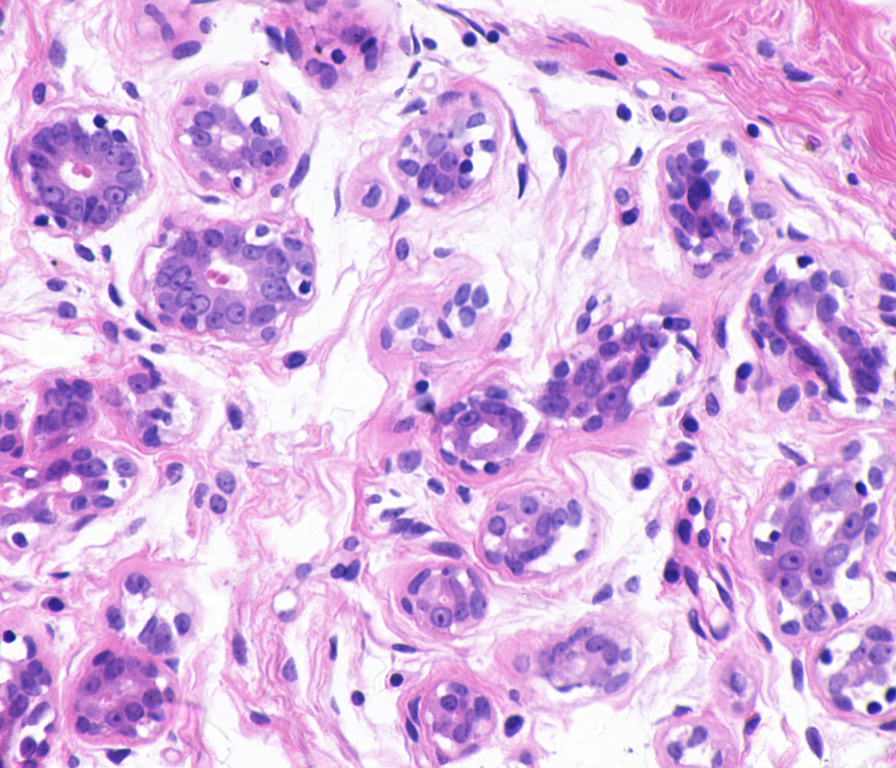
\includegraphics[width=\textwidth]{img/UCSBB (1).png}
        \caption{}
    \end{subfigure}\hfill
    \begin{subfigure}[b]{0.24\textwidth}
        \centering
        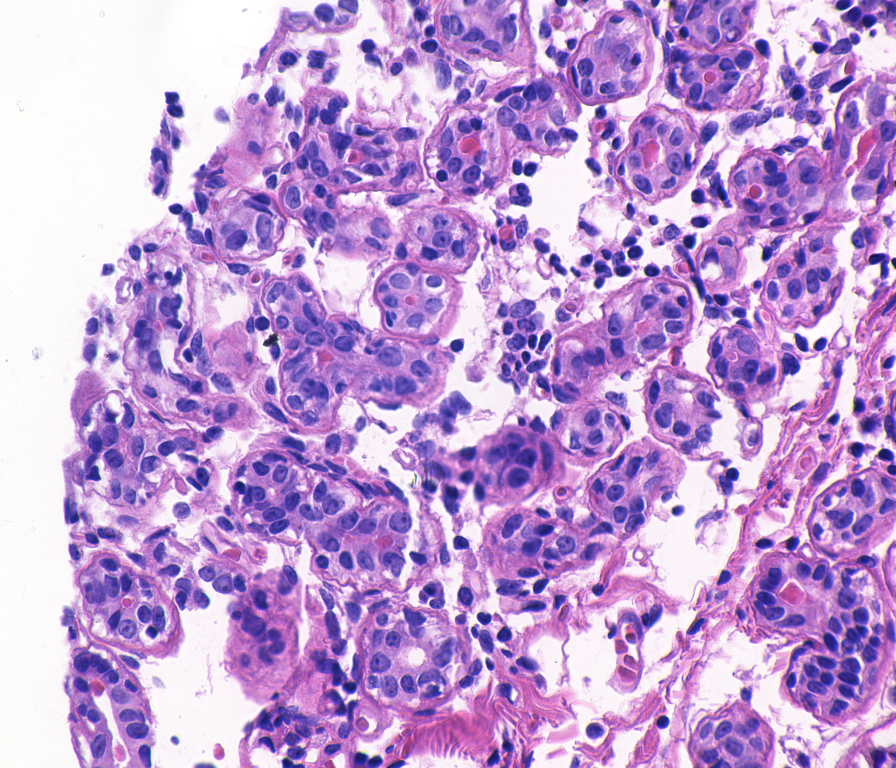
\includegraphics[width=\textwidth]{img/UCSBB (10).png}
        \caption{} 
    \end{subfigure}
    \hfill
    \begin{subfigure}[b]{0.24\textwidth}
        \centering
        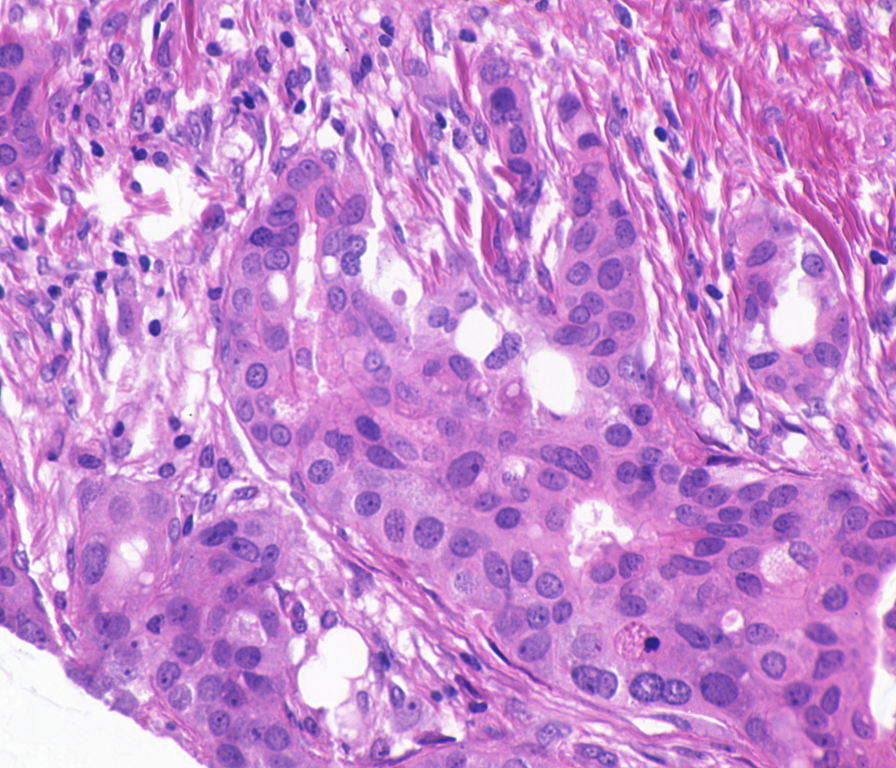
\includegraphics[width=\textwidth]{img/UCSBM (1).png}
        \caption{}
    \end{subfigure}
    \hfill
    \begin{subfigure}[b]{0.24\textwidth}
        \centering
        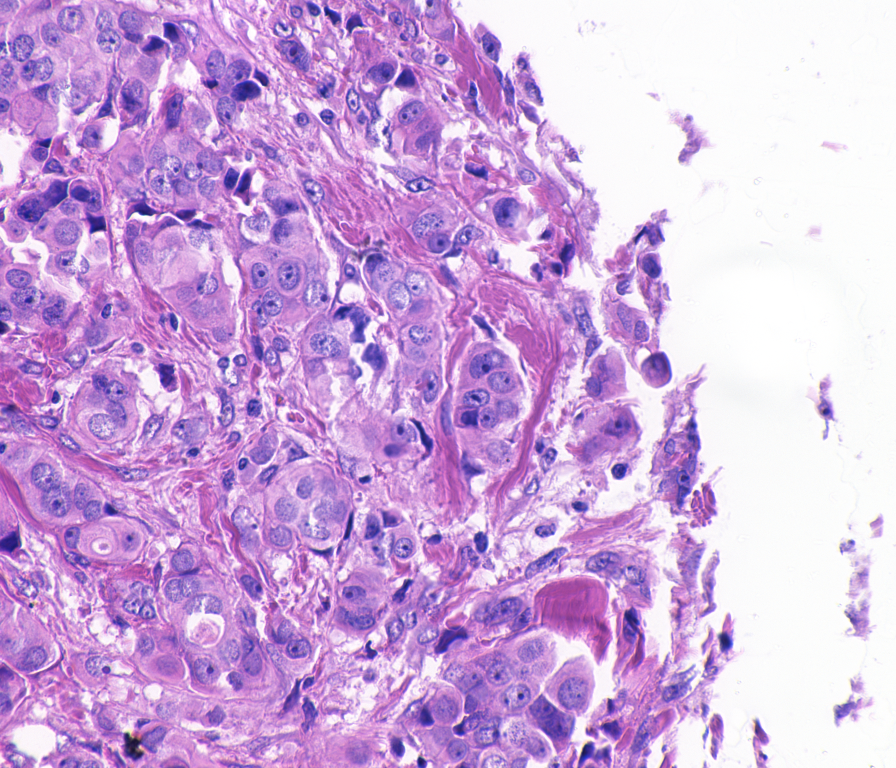
\includegraphics[width=\textwidth]{img/UCSBM (10).png}
        \caption{}
    \end{subfigure}

    \caption{Imagens exemplares do conjunto UCSB: (a, b) são tumores benignos e (c, d) são tumores malignos.}
    \label{fig:dataset-ucsb}
\end{figure}

O \textit{dataset} CR \cite{CR} contém 165 imagens RGB de tecido colorretal, obtidas a partir de 16 seções histológicas representativas de câncer colorretal nos estágios T3 e T4. O conjunto é levemente desbalanceado, com 74 imagens de tecido benigno e 91 de tecido maligno, e aquisições originais com resoluções de $567 \times 430$ a $775 \times 522$ pixels (Figura~\ref{fig:dataset-cr}).

\begin{figure}[htbp]
    \centering
    \begin{subfigure}[b]{0.24\textwidth}
        \centering
        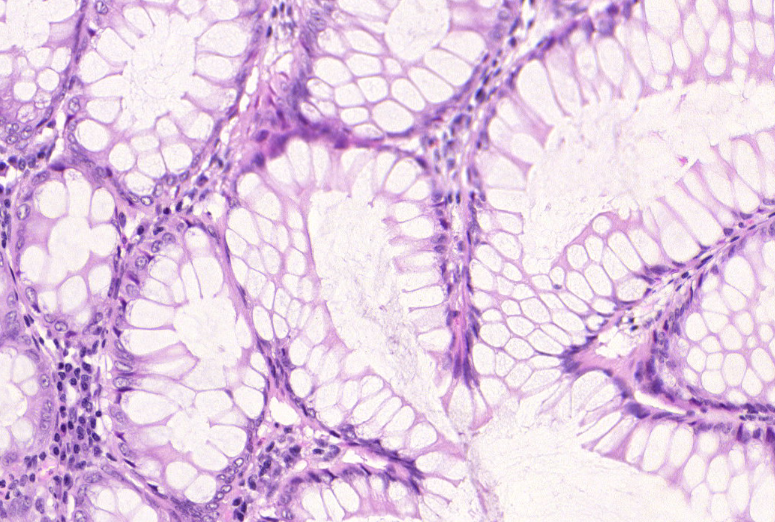
\includegraphics[width=\textwidth]{img/CRBenign (1).png}
        \caption{}
    \end{subfigure}\hfill
    \begin{subfigure}[b]{0.24\textwidth}
        \centering
        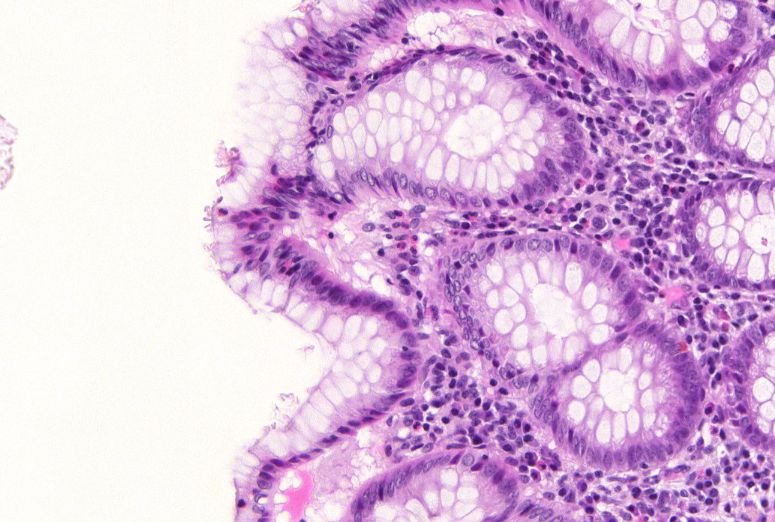
\includegraphics[width=\textwidth]{img/CRBenign (10).png}
        \caption{} 
    \end{subfigure}
    \hfill
    \begin{subfigure}[b]{0.24\textwidth}
        \centering
        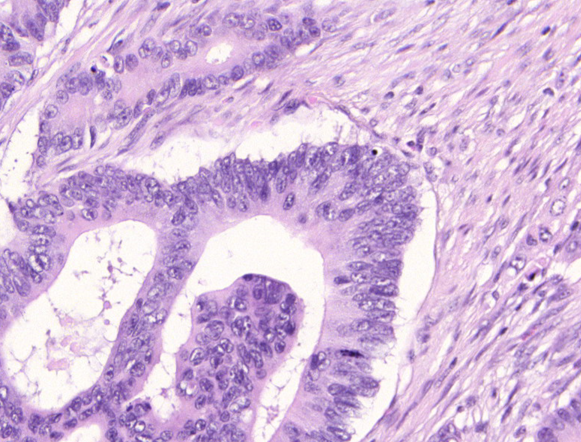
\includegraphics[width=\textwidth]{img/CRMalignant (1).png}
        \caption{}
    \end{subfigure}
    \hfill
    \begin{subfigure}[b]{0.24\textwidth}
        \centering
        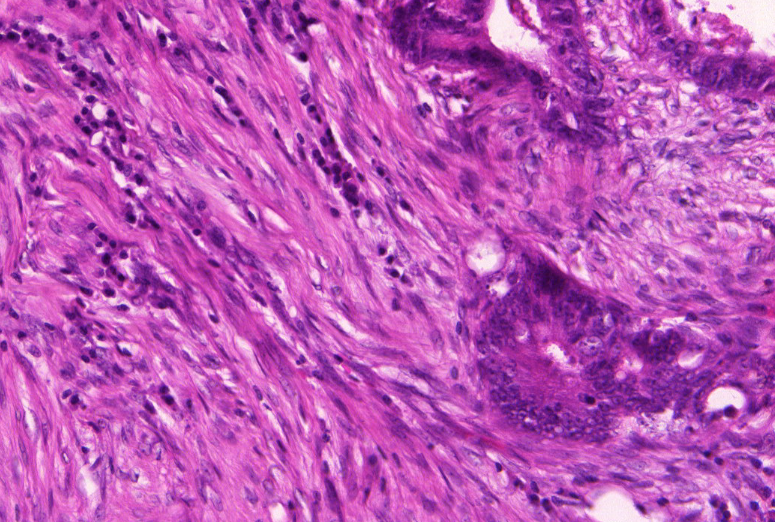
\includegraphics[width=\textwidth]{img/CRMalignant (10).png}
        \caption{}
    \end{subfigure}

    \caption{Imagens exemplares do conjunto CR: (a, b) são tecidos benignos e (c, d) são tecidos malignos.}
    \label{fig:dataset-cr}
\end{figure}

Os \textit{datasets} LA e LG \cite{iicbu2008} compreendem micrografias RGB de tecido hepático de camundongos. O LA tem como objetivo classificar a idade dos animais fêmeas em quatro grupos: um mês (100 imagens), seis meses (115), 16 meses (162) e 24 meses (151), totalizando 528 imagens. O LG contém 265 imagens para classificação de gênero, divididas em 150 machos e 115 fêmeas. As Figuras~\ref{fig:dataset-la} e \ref{fig:dataset-lg} apresentam amostras dos dois conjuntos.

\begin{figure}[htbp]
    \centering
    \begin{subfigure}[b]{0.24\textwidth}
        \centering
        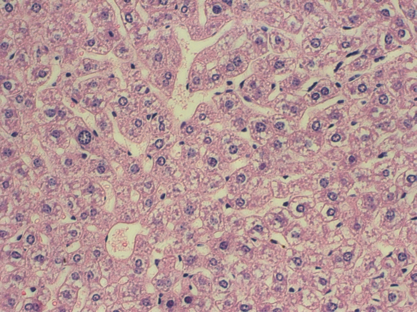
\includegraphics[width=\textwidth]{img/la 1.png}
        \caption{}
    \end{subfigure}\hfill
    \begin{subfigure}[b]{0.24\textwidth}
        \centering
        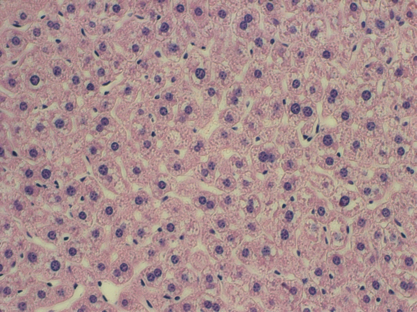
\includegraphics[width=\textwidth]{img/la 2.png}
        \caption{} 
    \end{subfigure}
    \hfill
    \begin{subfigure}[b]{0.24\textwidth}
        \centering
        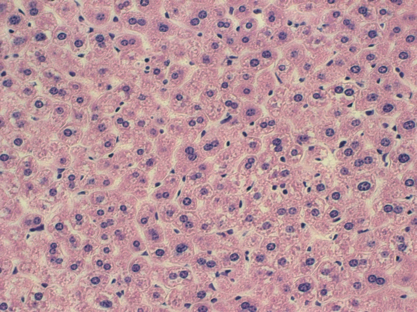
\includegraphics[width=\textwidth]{img/la 3.png}
        \caption{}
    \end{subfigure}
    \hfill
    \begin{subfigure}[b]{0.24\textwidth}
        \centering
        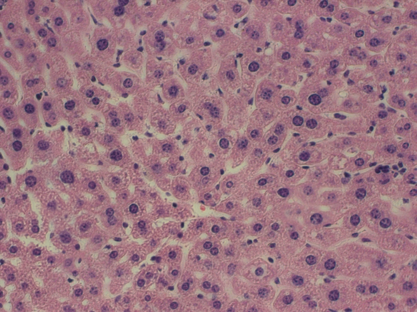
\includegraphics[width=\textwidth]{img/la 4.png}
        \caption{}
    \end{subfigure}

    \caption{Imagens de cada faixa etária dos camundongos do conjunto LA: um mês (a), seis meses (b), 16 meses (c) e 24 meses (d).}
    \label{fig:dataset-la}
\end{figure}

\begin{figure}[htbp]
    \centering
    \begin{subfigure}[b]{0.24\textwidth}
        \centering
        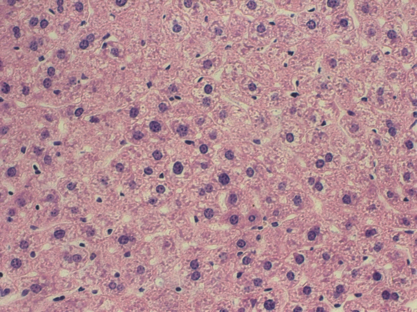
\includegraphics[width=\textwidth]{img/lg male 1.png}
        \caption{}
    \end{subfigure}\hfill
    \begin{subfigure}[b]{0.24\textwidth}
        \centering
        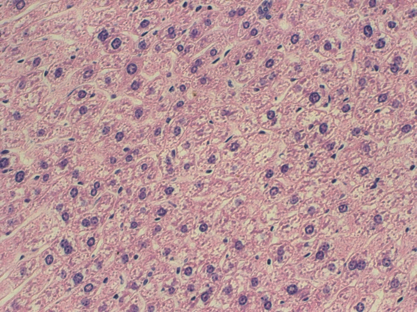
\includegraphics[width=\textwidth]{img/lg male 2.png}
        \caption{} 
    \end{subfigure}
    \hfill
    \begin{subfigure}[b]{0.24\textwidth}
        \centering
        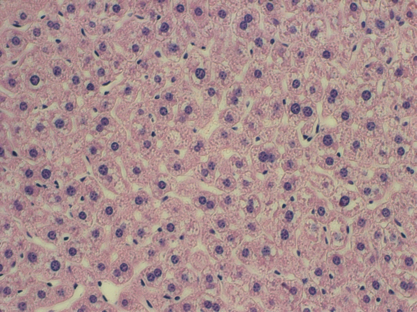
\includegraphics[width=\textwidth]{img/lg female 1.png}
        \caption{}
    \end{subfigure}
    \hfill
    \begin{subfigure}[b]{0.24\textwidth}
        \centering
        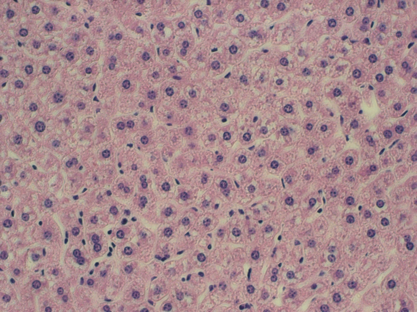
\includegraphics[width=\textwidth]{img/lg female 2.png}
        \caption{}
    \end{subfigure}

    \caption{Imagens de cada gênero dos camundongos do conjunto LG: (a, b) machos e (c, d) fêmeas.}
    \label{fig:dataset-lg}
\end{figure}

O \textit{dataset} NHL \cite{iicbu2008} contém 374 imagens RGB de linfoma não Hodgkin, distribuídas em três classes diagnósticas: leucemia linfocítica crônica (\textit{chronic lymphocytic leukemia}, CLL, 113 imagens), linfoma folicular (\textit{follicular lymphoma}, FL, 139 imagens) e linfoma de células do manto (\textit{mantle cell lymphoma}, MCL, 122 imagens). Diferentemente de aquisições realizadas em um único centro, o NHL reúne espécimes preparados por diferentes histologistas em diversos hospitais e laboratórios de histopatologia, apresentando marcantes variações de coloração e iluminação entre laboratórios (Figura~\ref{fig:dataset-nhl}). Esse conjunto foi incluído especificamente para avaliar a generalização dos modelos sob substancial variabilidade de domínio e cromática.

\begin{figure}[htbp]
    \centering
    \begin{subfigure}[b]{0.24\textwidth}
        \centering
        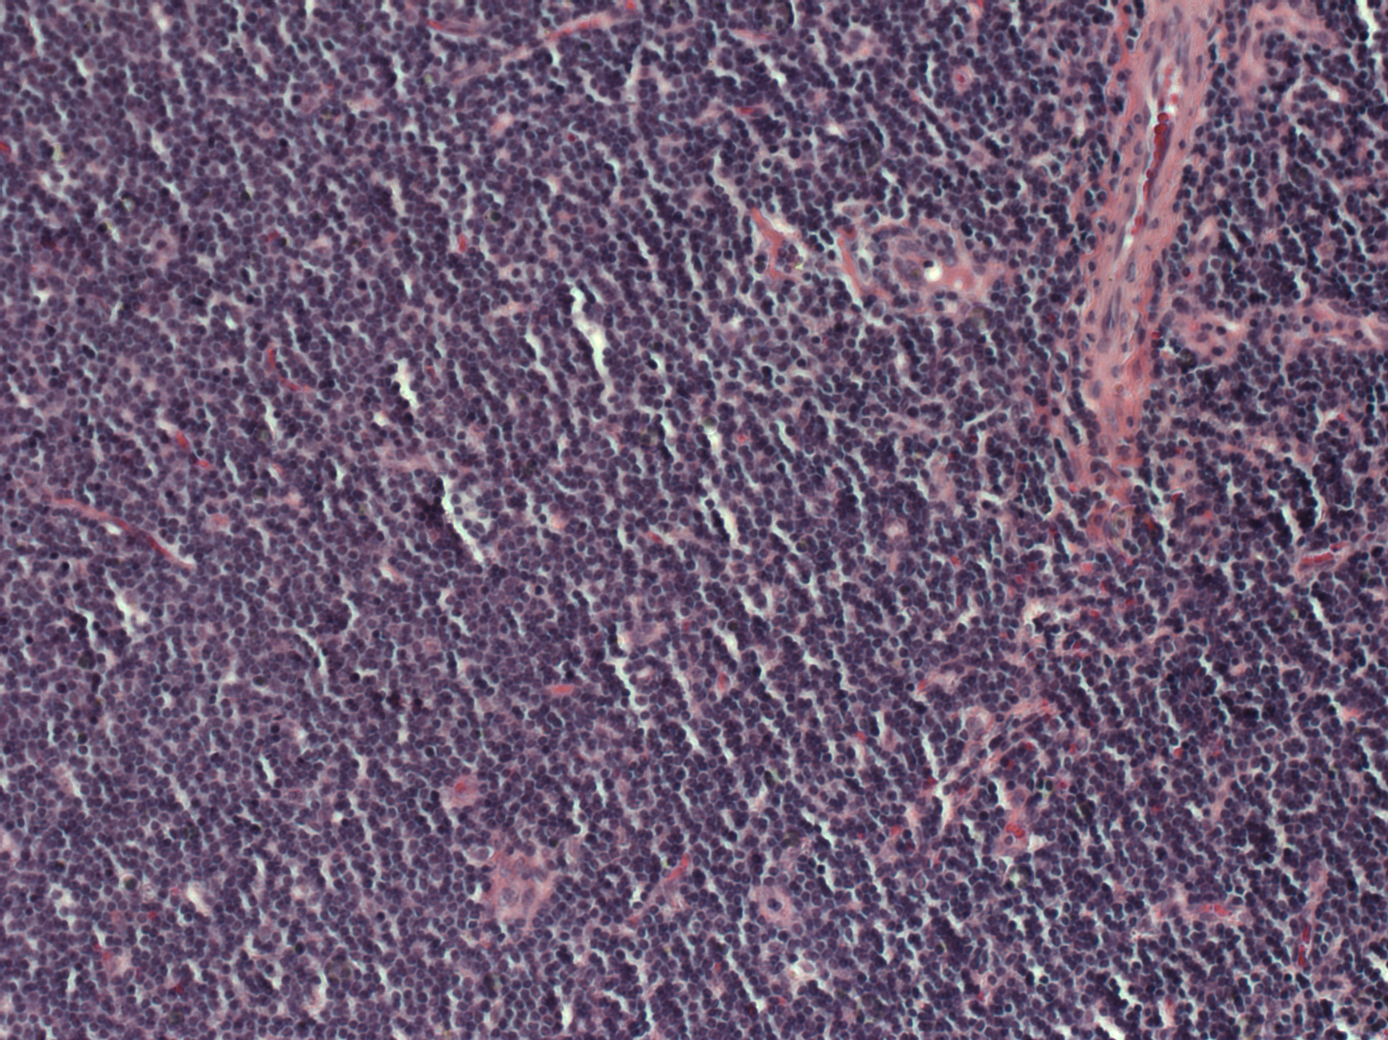
\includegraphics[width=\textwidth]{img/CLL (1).png}
        \caption{}
    \end{subfigure}\hfill
    \begin{subfigure}[b]{0.24\textwidth}
        \centering
        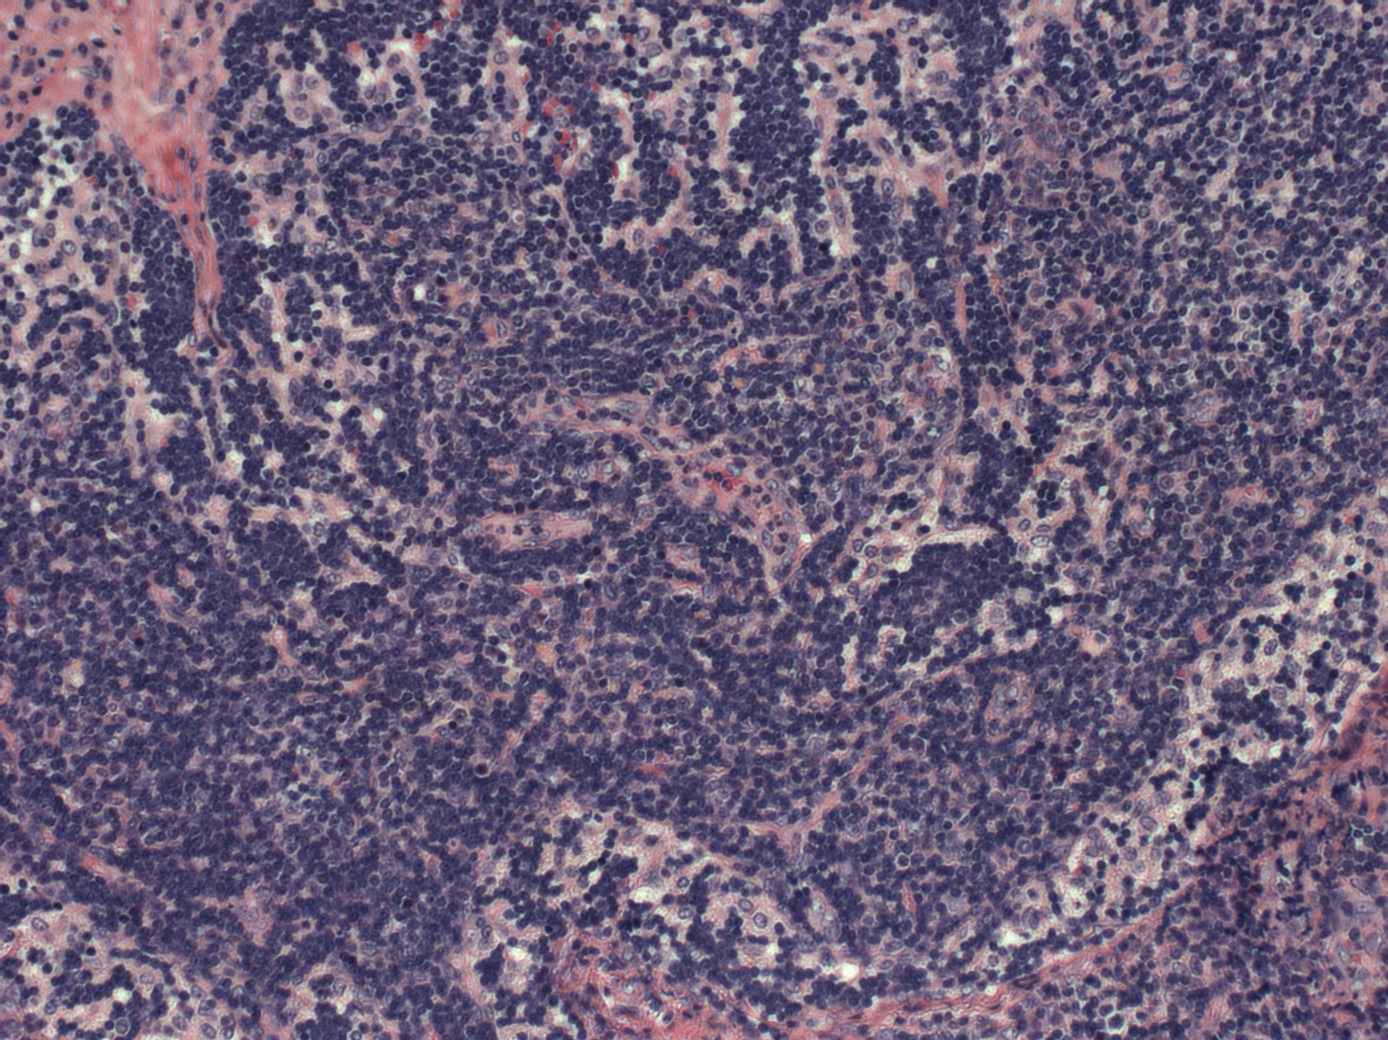
\includegraphics[width=\textwidth]{img/FL (1).png}
        \caption{} 
    \end{subfigure}
    \hfill
    \begin{subfigure}[b]{0.24\textwidth}
        \centering
        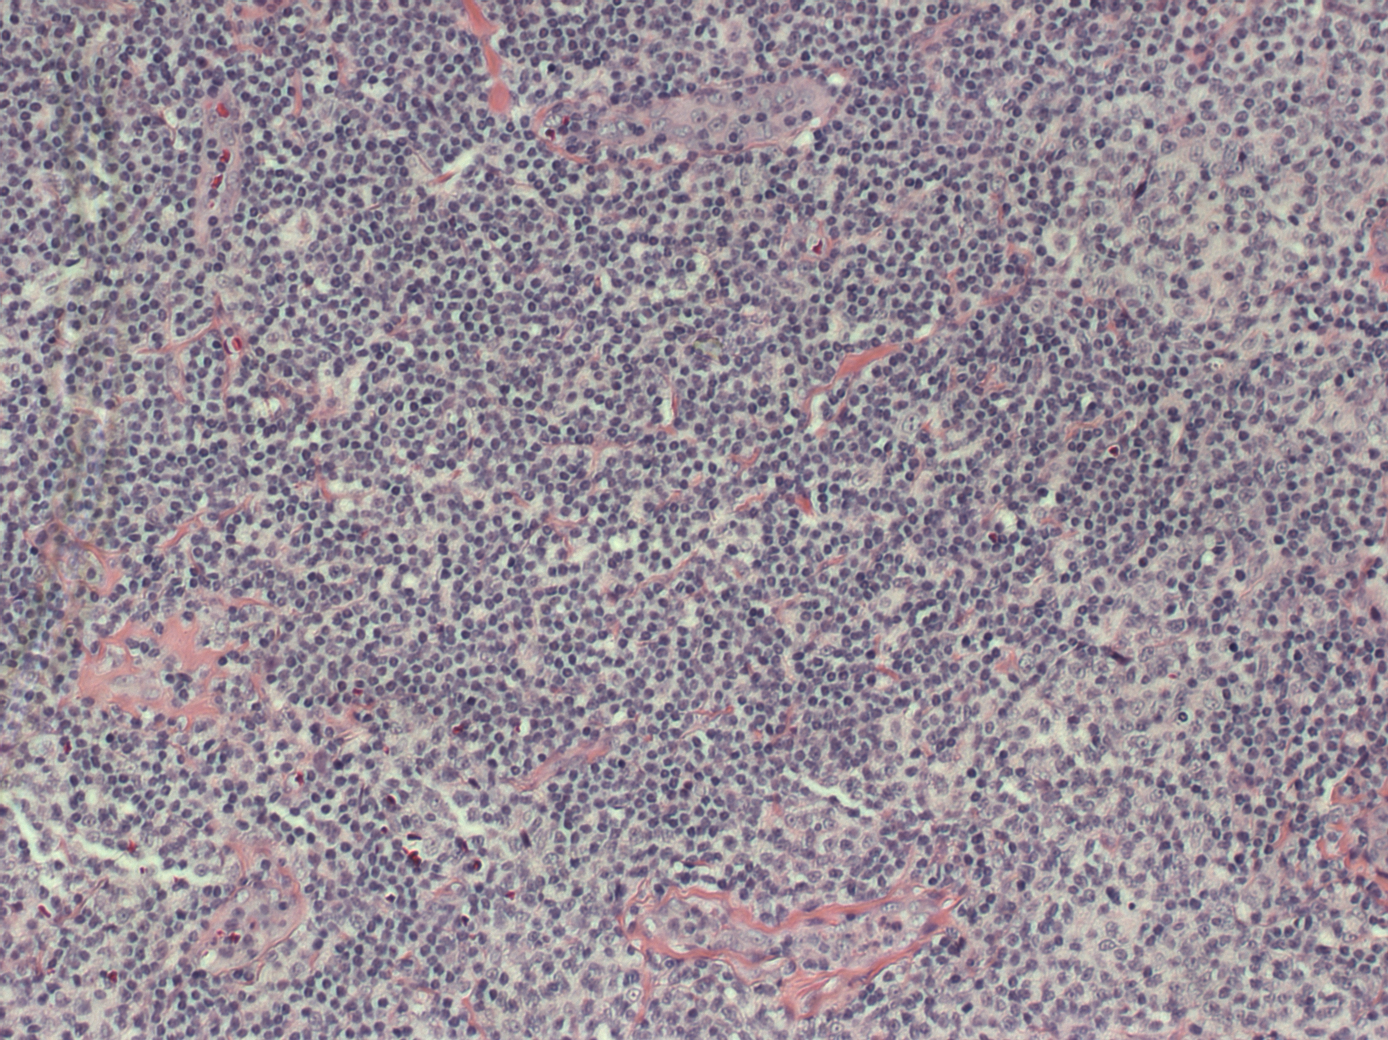
\includegraphics[width=\textwidth]{img/MCL (1).png}
        \caption{}
    \end{subfigure}

    \caption{Amostras do conjunto NHL: (a) CLL, (b) FL e (c) MCL.}
    \label{fig:dataset-nhl}
\end{figure}


\section{\textit{Two-Stream Network}}
\label{sec:duas-vias}

A arquitetura proposta, ilustrada na Figura~\ref{fig:pipeline_tcc}, consiste em uma rede de dupla via (\textit{Two-Stream Network}) destinada à classificação de imagens histopatológicas. O modelo combina duas representações complementares da imagem: uma representação topológica, construída a partir de medidas de redes complexas e processada por uma rede neural recorrente, e uma representação visual, extraída por uma arquitetura híbrida baseada em convoluções e mecanismos de atenção. As duas vias operam de forma independente durante a extração de características, e suas representações são integradas posteriormente por concatenação, seguida de um perceptron multicamadas (\textit{Multilayer Perceptron} -- MLP).

A separação dos fluxos permite explorar diferentes propriedades da imagem. A via topológica descreve as relações entre pixels e suas variações em diferentes escalas espaciais, enquanto a via visual aprende representações diretamente dos padrões presentes na imagem RGB. Essa organização é fundamentada em arquiteturas de dupla via empregadas na literatura para separar domínios de aprendizado conjunto (\textit{joint learning}) \cite{yousaf2024twostream,wang2023stnet}. A combinação de descritores calculados explicitamente com características profundas minimiza a dependência de grandes volumes de dados, abordando restrições comuns na classificação de imagens histopatológicas \cite{huang2022fusing}.

O processamento é dividido em quatro etapas principais: (i) extração de características texturais por meio de redes complexas e codificação temporal por uma rede recorrente; (ii) extração de características visuais pela MobileViT; (iii) concatenação dos vetores resultantes; e (iv) classificação da matriz conjunta pelo MLP. A predição final resulta de uma avaliação simultânea das informações morfológicas e locais.

\subsection{Extração de \textit{features} texturais}
\label{subsec:ext-tex}

A primeira via representa a textura da imagem por meio de medidas topológicas obtidas de redes complexas. A abordagem transforma cada pixel em um vértice de um grafo, estabelecendo arestas entre pixels vizinhos com base em suas posições e intensidades. A conversão das imagens para redes complexas permite quantificar características topológicas que algoritmos baseados em matrizes de vizinhança convencionais não processam diretamente \cite{BACKES2013168,ribas2020fusion,ribas2024colorspectral}.

Redes direcionadas e ponderadas são construídas para cada amostra, sendo as conexões delimitadas por um raio máximo $r_{\max}$. O peso da aresta reflete a diferença absoluta de intensidade, e sua direção indica o gradiente local entre os pixels. Considerando o formato RGB, adota-se a configuração \textit{full}, a qual estabelece ligações tanto intra quanto intercanais para analisar conjuntamente as mudanças de textura e cromaticidade \cite{Scabini_2020,CNT}.

Quatro grandezas topológicas (grau de saída, grau de entrada, força de saída e força de entrada) são calculadas para cada vértice. O raio máximo estipulado foi $r_{\max}=10$. A escolha resulta da observação do pico de ganho de informação aferido pelas entropias de Shannon e amostral em avaliações prévias da base de dados, estando alinhada aos achados da literatura sobre análise multiescala em grafos coloridos \cite{ribas2024colorspectral,CNT}. 

Para transformar essas matrizes em um vetor representativo de dimensão fixa para cada raio $r$, a média global e o desvio padrão global das quatro medidas são calculados para cada um dos três canais da imagem. A agregação dessas duas medidas estatísticas produz 24 características estáticas para cada incremento do raio \cite{ribas2024colorspectral}. A representação ordenada desse processo compõe a sequência de entrada:

\begin{equation}
X_{\mathrm{top}} =
[x_1,x_2,\ldots,x_{10}],
\label{eq:sequencia-topologica}
\end{equation}

em que cada passo da sequência corresponde ao vetor $x_r \in \mathbb{R}^{24}$.

O processamento dessa evolução espacial é executado por uma rede recorrente do tipo \textit{Long Short-Term Memory} Bidirecional (BiLSTM). A leitura bidirecional percorre as representações do micro (raio 1) para o macro (raio 10) e em sentido inverso, uma estratégia adotada na extração de sequências espaço-temporais em modelos de dupla via para maximizar a captura de padrões \cite{yousaf2024twostream,hochreiter1997long}. A BiLSTM foi instanciada com uma camada oculta de 128 unidades em cada sentido de leitura. A concatenação dos estados ocultos produzidos em ambas as direções forma o \textit{embedding} topológico $z_{\mathrm{top}} \in \mathbb{R}^{256}$, o qual é repassado ao módulo de fusão.

\subsection{Extração via MobileViT}
\label{subsec:ext-hibrido}

A via paralela obtém atributos visuais diretamente da matriz RGB utilizando a MobileViT, uma arquitetura híbrida projetada para fundir operações de convolução e mecanismos de atenção global de forma eficiente. O processamento combinado é aplicado na histopatologia para assimilar detalhes microcelulares por meio das convoluções e avaliar o tecido em larga escala pelos blocos de \textit{transformer} \cite{mehta2022mobilevit,oliveira2025hybrid}.

A versão implementada para a extração de características é a MobileViT-S (Small). A adoção desta variante pauta-se na capacidade de gerar representações discriminativas sem exceder restrições computacionais em bases de dados limitadas \cite{mehta2022mobilevit}. O modelo recebe os dados de entrada na resolução padronizada de $256 \times 256$ pixels. Para utilizar a arquitetura como um extrator puro em \textit{transfer learning}, a camada densa de classificação originalmente concebida no topo da rede foi suprimida.

As ativações produzidas pelo último bloco convolucional são submetidas a uma camada de agrupamento médio global (\textit{Global Average Pooling}). Esta operação condensa a dimensionalidade espacial dos mapas de características em um tensor linear. Sendo $I$ a imagem processada e $f_{\mathrm{vis}}(\cdot)$ o codificador visual, o mapeamento é expresso por:

\begin{equation}
z_{\mathrm{vis}} = f_{\mathrm{vis}}(I),
\label{eq:embedding-visual}
\end{equation}

onde $z_{\mathrm{vis}} \in \mathbb{R}^{640}$ representa o \textit{embedding} visual.

A arquitetura visual é inicializada com os pesos da ImageNet, permitindo a reutilização das respostas de filtragem primárias otimizadas durante as etapas de treinamento do modelo proposto. O vetor de 640 dimensões resultante é transmitido em paralelo para a camada de integração.

\subsection{Fusão Tardia}
\label{sec:late-fusion}

A fusão tardia (\textit{Late Fusion}) constitui a etapa na qual os \textit{embeddings} derivados da via topológica e da via visual são combinados no mesmo espaço dimensional. A junção dessas representações independentes a nível de \textit{features} evita interferências recíprocas na aprendizagem local dos pesos, procedimento aplicado com eficácia na análise de câncer de próstata com características manuais e profundas \cite{huang2022fusing,baltrusaitis2019multimodal}.

A combinação simples dos tensores expõe a rede ao problema da divergência de magnitude. Os valores provenientes da rede BiLSTM são matematicamente delimitados no intervalo $[-1, 1]$ em função da tangente hiperbólica de sua célula de memória. Os dados extraídos pela MobileViT passam por ativações não limitadas (\textit{ReLU} ou \textit{Swish}). A discrepância numérica leva os atributos de maior escala a anularem a influência dos atributos menores durante a propagação do erro. Para garantir a paridade na representação conjunta, os vetores $z_{\mathrm{top}}$ e $z_{\mathrm{vis}}$ são regularizados por uma camada de normalização de ativações (\textit{Layer Normalization}) imediatamente antes da junção \cite{huang2022fusing}.

A construção do vetor unificado é executada pela concatenação dos tensores normalizados:

\begin{equation}
z_{\mathrm{fusão}} =
\left[z_{\mathrm{top}}\,\Vert\,z_{\mathrm{vis}}\right]
\in\mathbb{R}^{896},
\label{eq:fusao-concat}
\end{equation}

em que o símbolo $\Vert$ indica a operação matemática de alinhamento sequencial. O tensor resultante carrega a somatória das representações da BiLSTM ($d_t = 256$) e da MobileViT-S ($d_v = 640$). O vetor completo é alimentado na etapa de decisão não linear do modelo.

\subsection{Classificador MLP}
\label{sec:mlp}

A discriminação das classes histopatológicas baseada na matriz fundida é executada por um perceptron multicamadas (MLP). O classificador mapeia os 896 atributos recebidos e estabelece relações estatísticas entre a forma visual do tecido e a distribuição estrutural de seu grafo \cite{rumelhart1986learning}. 

A rede foi projetada com uma camada oculta contendo 512 neurônios. A transformação inicial dos dados é modelada pela equação:

\begin{equation}
h =
\operatorname{ReLU}
\left(W_1 z_{\mathrm{fusão}} + b_1\right),
\label{eq:mlp-hidden}
\end{equation}

em que a função de ativação linear retificada (\textit{ReLU}) introduz não linearidade e gera a representação profunda $h$. A arquitetura compacta atua na prevenção do sobreajuste. Como técnica adicional de regularização direcionada aos cenários de dados exíguos encontrados nos conjuntos UCSB e CR, uma camada \textit{Dropout} configurada com retenção de 50\% (probabilidade de 0,5) processa as ativações produzidas \cite{srivastava2014dropout, nawaz2025ard}.

As respostas estabilizadas alimentam a camada terminal do classificador. A camada de saída é instanciada com uma dimensão $C$, condizente ao número de categorias de cada base de dados (variando entre 2 a 4 neurônios). Os escores brutos são processados conforme a equação:

\begin{equation}
\hat{y} =
\operatorname{softmax}
\left(W_2 h + b_2\right).
\label{eq:mlp-output}
\end{equation}

A função \textit{softmax} distribui os resultados em um escopo normalizado, gerando o vetor de probabilidade $\hat{y}$ relativo à classificação final da amostra de tecido.

\section{Protocolo de treinamento}
\label{sec:protocolo}

A arquitetura proposta é treinada de forma conjunta (\textit{end-to-end}). O fluxo de processamento atualiza simultaneamente os parâmetros da rede MobileViT-S, da rede recorrente e do perceptron multicamadas. A divergência entre as predições e os rótulos verdadeiros é calculada pela função de perda de entropia cruzada. O otimizador AdamW é empregado para a atualização dos pesos, configurado com uma taxa de aprendizado inicial de $1 \times 10^{-4}$. A rede visual é submetida a ajuste fino a partir de pesos pré-treinados, enquanto os parâmetros das vias sequencial e de decisão são inicializados aleatoriamente.

A avaliação do modelo adota a validação cruzada estratificada com 10 partições (10-\textit{fold}) \cite{kohavi1995study}. O conjunto de dados é dividido em 10 subconjuntos independentes. Em cada iteração, nove partições são utilizadas para o treinamento da rede e uma partição forma o conjunto de teste isolado. A divisão estratificada preserva a proporção original das classes em todas as partições. O resultado de desempenho do modelo corresponde à média aritmética das métricas obtidas nas 10 iterações.

\subsection{Métricas}

O desempenho da classificação é quantificado pelas métricas de Acurácia, F1-Score e Área Sob a Curva ROC (AUC-ROC). A Acurácia contabiliza a proporção global de predições corretas. O F1-Score estabelece a média harmônica entre a precisão e a sensibilidade, fornecendo uma avaliação adequada para conjuntos de dados com desbalanceamento de classes, como o \textit{dataset} CR. A métrica AUC-ROC afere a capacidade do classificador em distinguir entre as categorias ao longo de diferentes limiares de decisão. O desempenho da rede de dupla via é comparado diretamente aos resultados obtidos pelas técnicas de extração clássica (GLCM, LBP e HOG) submetidas à mesma arquitetura de classificação e ao mesmo particionamento de dados.

\section{Configuração de ambiente}
\label{sec:env}

Os experimentos foram desenvolvidos na linguagem Python. A implementação da rede neural de dupla via, a extração de características e a otimização dos pesos foram executadas utilizando o \textit{framework} PyTorch. O cálculo das matrizes topológicas e a extração dos descritores clássicos empregaram bibliotecas de processamento de imagens e análise de grafos. O treinamento e a inferência dos modelos foram acelerados por meio de unidades de processamento gráfico (GPUs).
